\documentclass{beamer}
\usepackage{graphicx}
\usepackage{tikz}
\usetikzlibrary{shapes,arrows}
\usepackage{tikz}
\usetheme{default}
%\usecolortheme{seahorse}

  \setbeamertemplate{footline}[page number]
\setbeamertemplate{navigation symbols}{}
\setbeamertemplate{frametitle}[default][center]
\setbeamerfont{frametitle}{shape=\scshape}

\usepackage{color}

\usepackage{media9}%
\newcommand{\includemovie}[3]{%
\includemedia[%
width=#1,height=#2,%
activate=pagevisible,%
deactivate=pageclose,%
addresource=#3,%
flashvars={%
src=#3 % same path as in addresource!
&autoPlay=true % default: false; if =true, automatically starts playback after activation (see option ?activation)?
&loop=true % if loop=true, media is played in a loop
&controlBarAutoHideTimeout=0 %  time span before auto-hide
}%
]{}{StrobeMediaPlayback.swf}}%


{\title{\textsc{Numerical Methods-Lecture IX: Reinforcement Learning} \\ \ \\ \tiny (See Powell Chapter 10)}
\author{Trevor S. Gallen}
\date{}

\begin{document}

\begin{frame}
\titlepage
\end{frame}

\begin{frame}
\frametitle[alignment=center]{Motivation}
\begin{itemize}
\item Previously, this lecture was devoted to quadrature, and specifically how to integrate sampling from Chebyshev nodes
\bigskip
\item While valuable, it may be going out of style relative to modern methods
\bigskip
\item Instead, we'll talk about Reinforcement Learning
\bigskip
\item Could have had a whole course, but I want to give you the motivation and a crash course
\end{itemize}
\end{frame}


\begin{frame}
\frametitle[alignment=center]{Neural Networks}
\begin{itemize}
\item Neural networks, for our purposes, are just very very flexible nonlinear functional forms
\smallskip
\item Have $y^{data}$ and want to fit $f(x|\theta)$ to it
\smallskip
\item One way of producing a flexible function with easy derivatives (for fitting) is to stack logit functions 
\smallskip
\item Idea:  $X=[x_1,x_2,...]$ gets fed into multiple logits $f_1(X)$, $f_2(X)$, $f_3(X)$, each with its own logit weight on $X$: $\beta_1^f$, $\beta_2^f$, $\beta_3^f$.
\smallskip
\item The outputs of these three (+) logits then (possibly) get fed into another set of logits, $g_1(f_1,f_2,f_3)$, $g_2(f_1,f_2,f_3)$, each with their own set of weights $\beta^g_1$...
\smallskip
\item Eventually these are summed up or scaled to a single (or multiple!) output, such as $y^{fit}$
\smallskip
\item For most uses, NN just find $\theta$ like we would in any fitting problem, but use gradient descent (chain rule!) rather than Newton's method (too many cross-derivatives + many local minima)
\end{itemize}
\end{frame}

\begin{frame}
\frametitle[alignment=center]{Neural Networks}
\begin{itemize}
\item Concrete example:  want to approximate $f(x)$
\bigskip
\item Suggestion:  one set of five logits, whose sum is then scaled:
$$f(x)\approx \alpha_{L2}+\left(\sum_{i=1}^5 \beta_{L2,i}\frac{1}{1+e^{-(\alpha_{1,i}+\beta_{L1,i}x)}}\right)$$
\item A little hard to read!  
\bigskip
\item See Simple\_5\_Main.m, and then Simple\_N\_Main.m for N logits
\end{itemize}
\end{frame}


\begin{frame}
\frametitle[alignment=center]{Neural Networks: 5 Logit+Linear Approx}
\begin{figure}
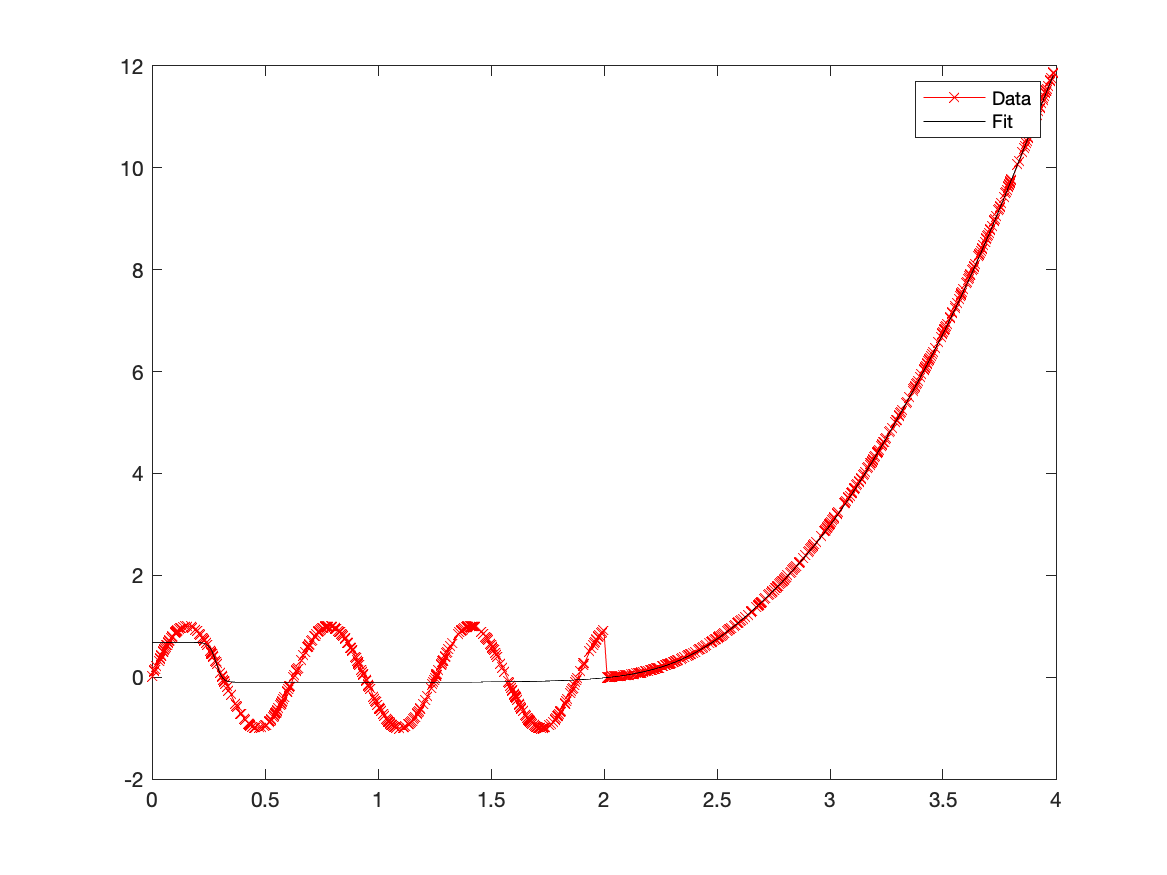
\includegraphics[scale=0.5]{NN_Example/Fig_Shallow_5.png}
\end{figure}
\end{frame}

\begin{frame}
\frametitle[alignment=center]{Neural Networks: 1 Logit+Linear Approx}
\begin{figure}
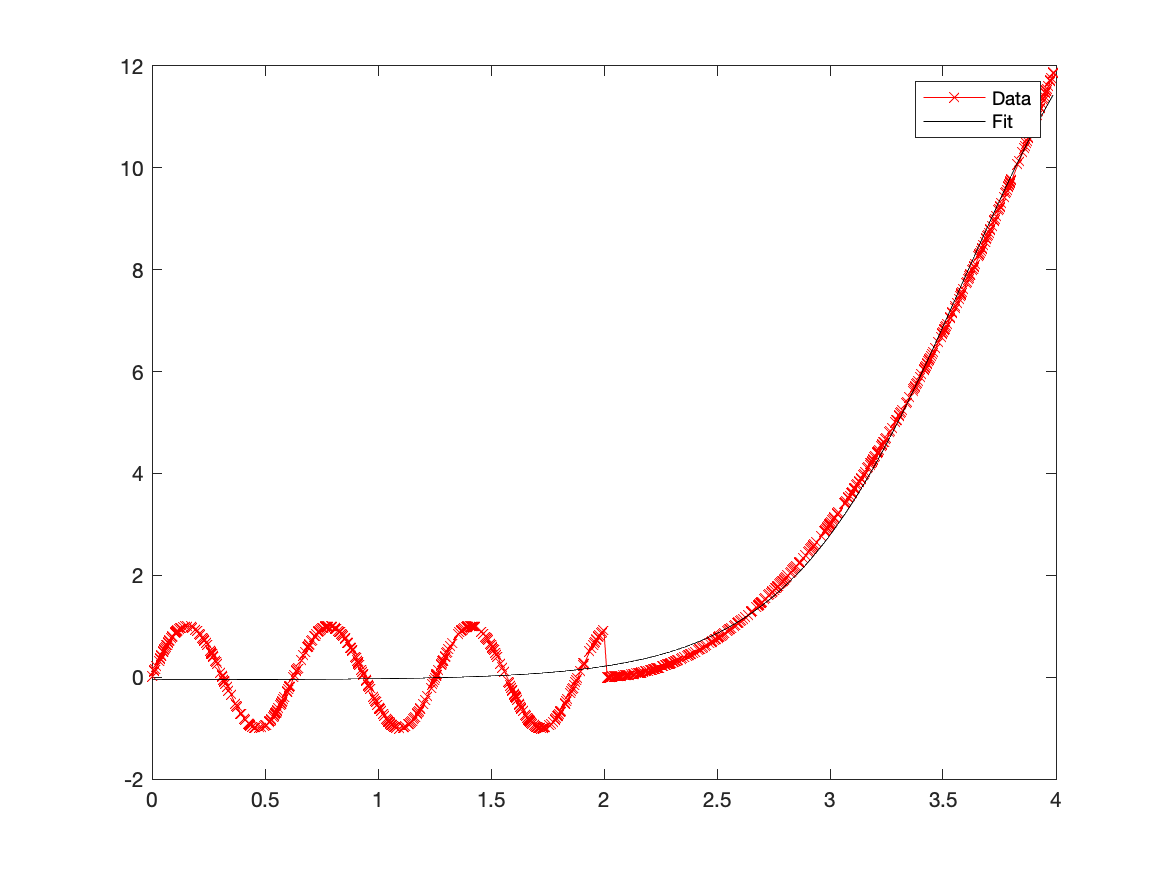
\includegraphics[scale=0.5]{NN_Example/Fig_Shallow_1.png}
\end{figure}
\end{frame}

\begin{frame}
\frametitle[alignment=center]{Neural Networks: 2 Logit+Linear Approx}
\begin{figure}
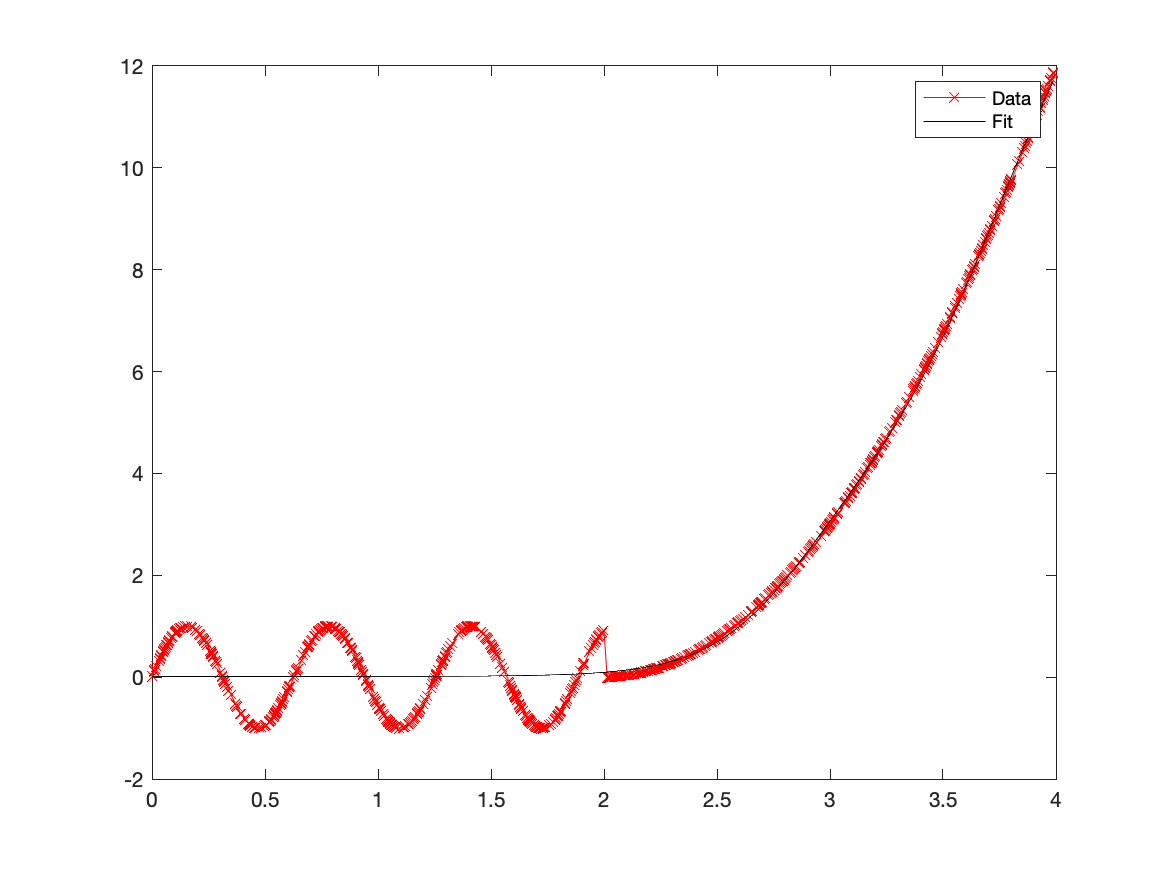
\includegraphics[scale=0.5]{NN_Example/Fig_Shallow_2.png}
\end{figure}
\end{frame}

\begin{frame}
\frametitle[alignment=center]{Neural Networks: 3 Logit+Linear Approx}
\begin{figure}
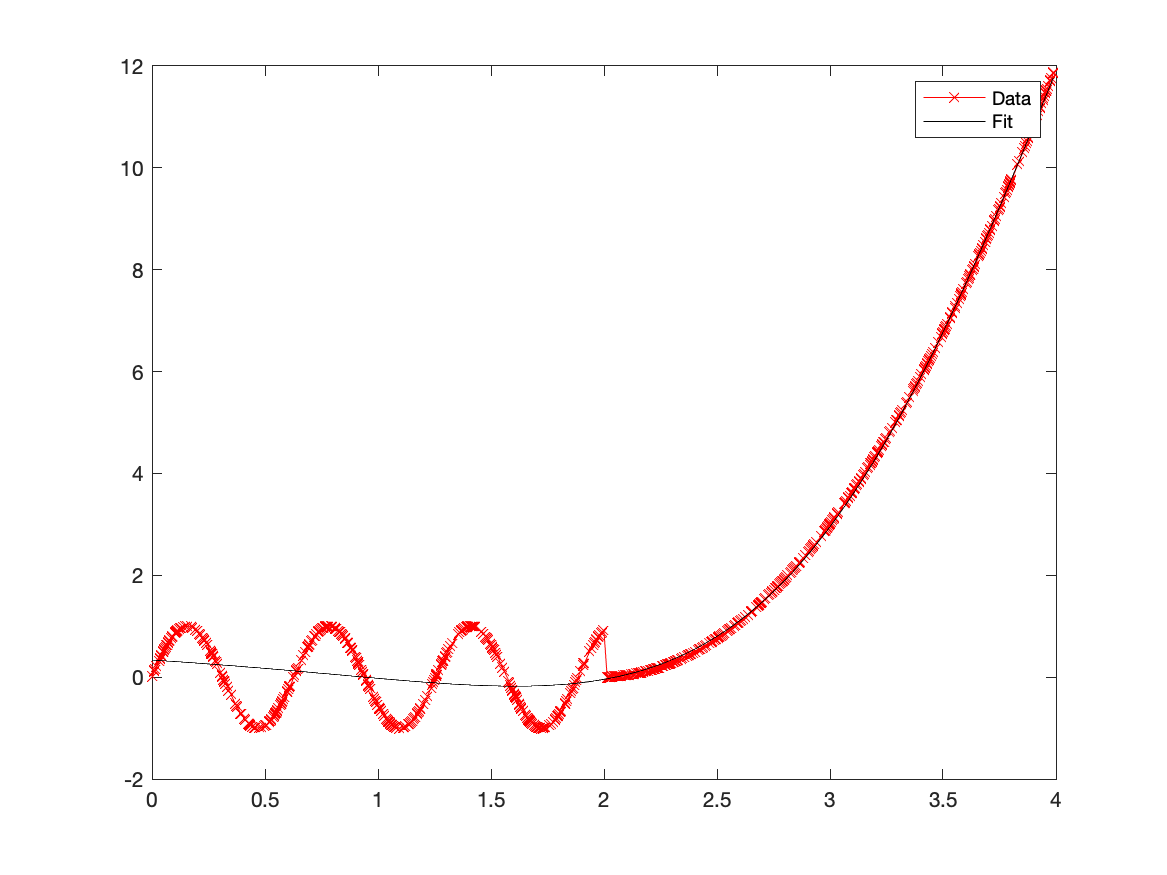
\includegraphics[scale=0.5]{NN_Example/Fig_Shallow_3.png}
\end{figure}
\end{frame}

\begin{frame}
\frametitle[alignment=center]{Neural Networks: 4 Logit+Linear Approx}
\begin{figure}
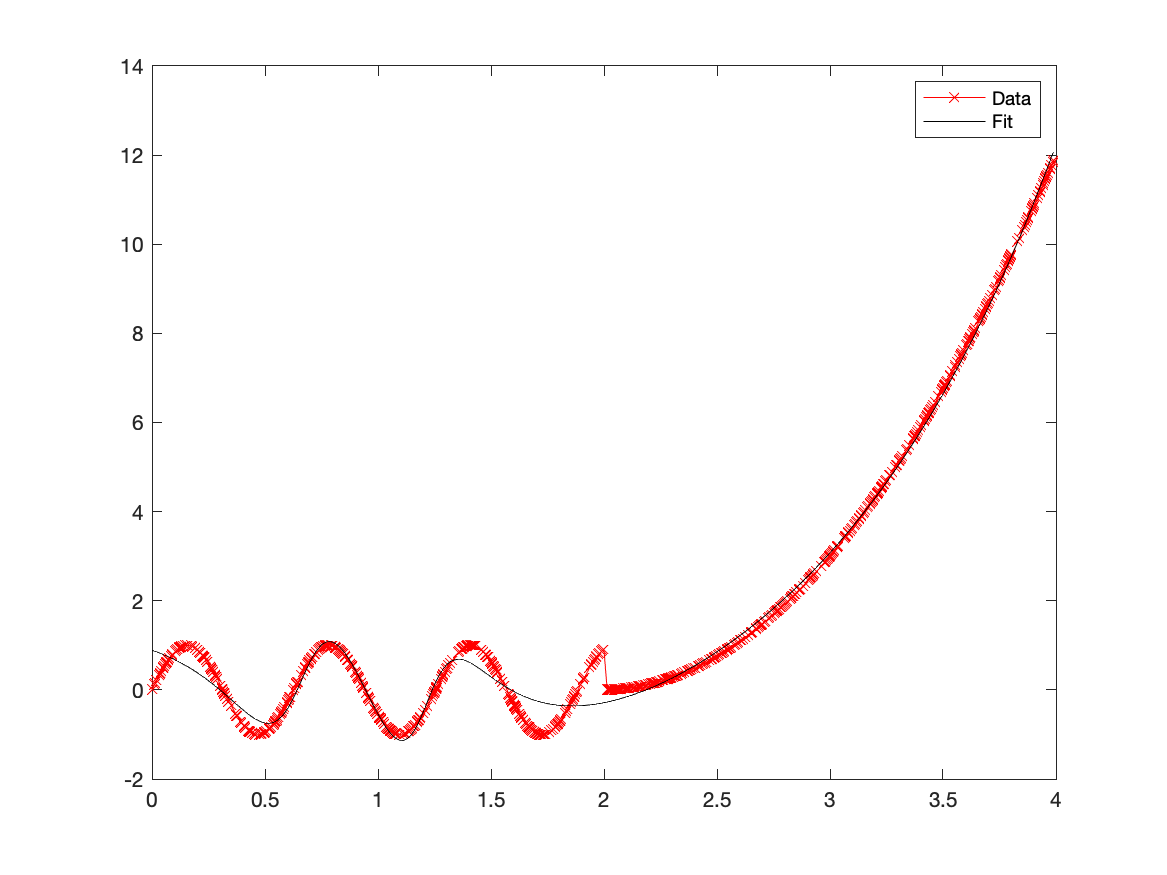
\includegraphics[scale=0.5]{NN_Example/Fig_Shallow_4.png}
\end{figure}
\end{frame}


\begin{frame}
\frametitle[alignment=center]{Neural Networks: 6 Logit+Linear Approx}
\begin{figure}
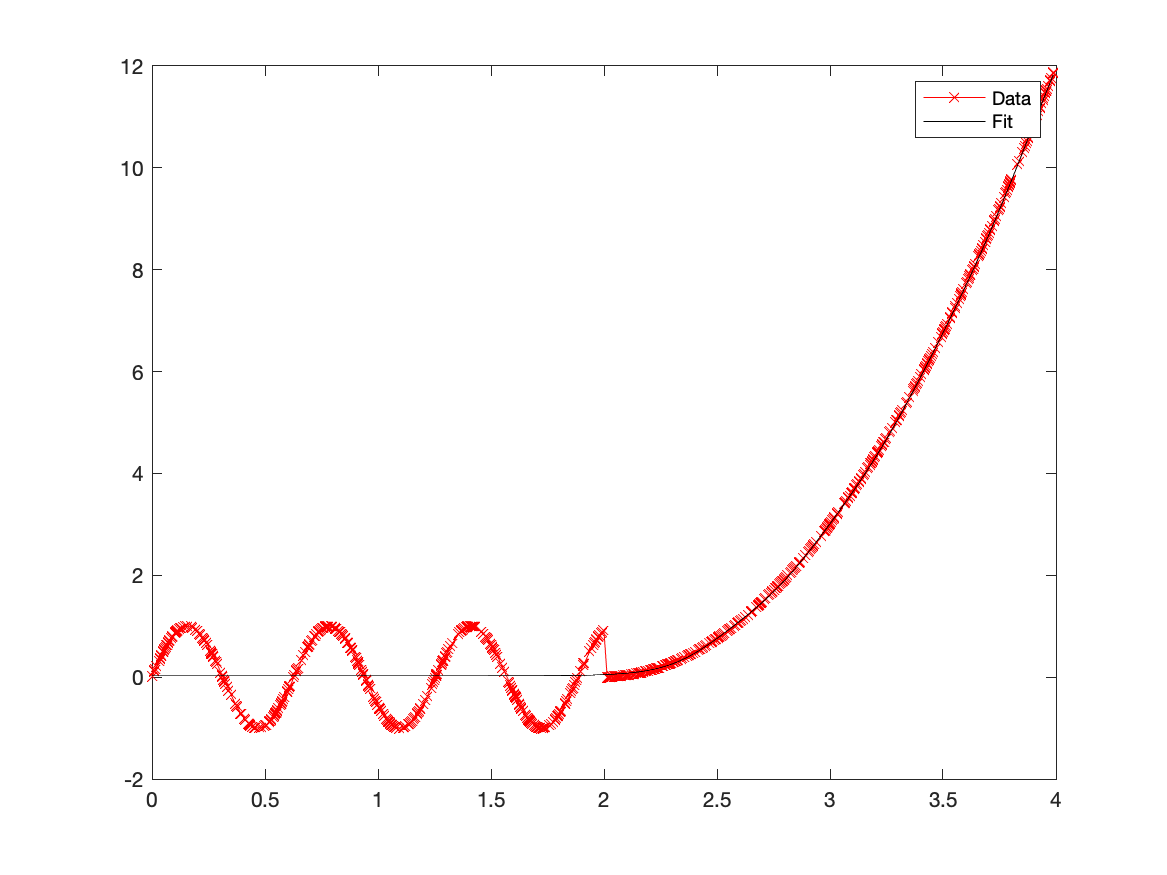
\includegraphics[scale=0.5]{NN_Example/Fig_Shallow_6.png}
\end{figure}
Got stuck at local minima!  (Bad!)
\end{frame}

\begin{frame}
\frametitle[alignment=center]{Neural Networks: 7 Logit+Linear Approx}
\begin{figure}
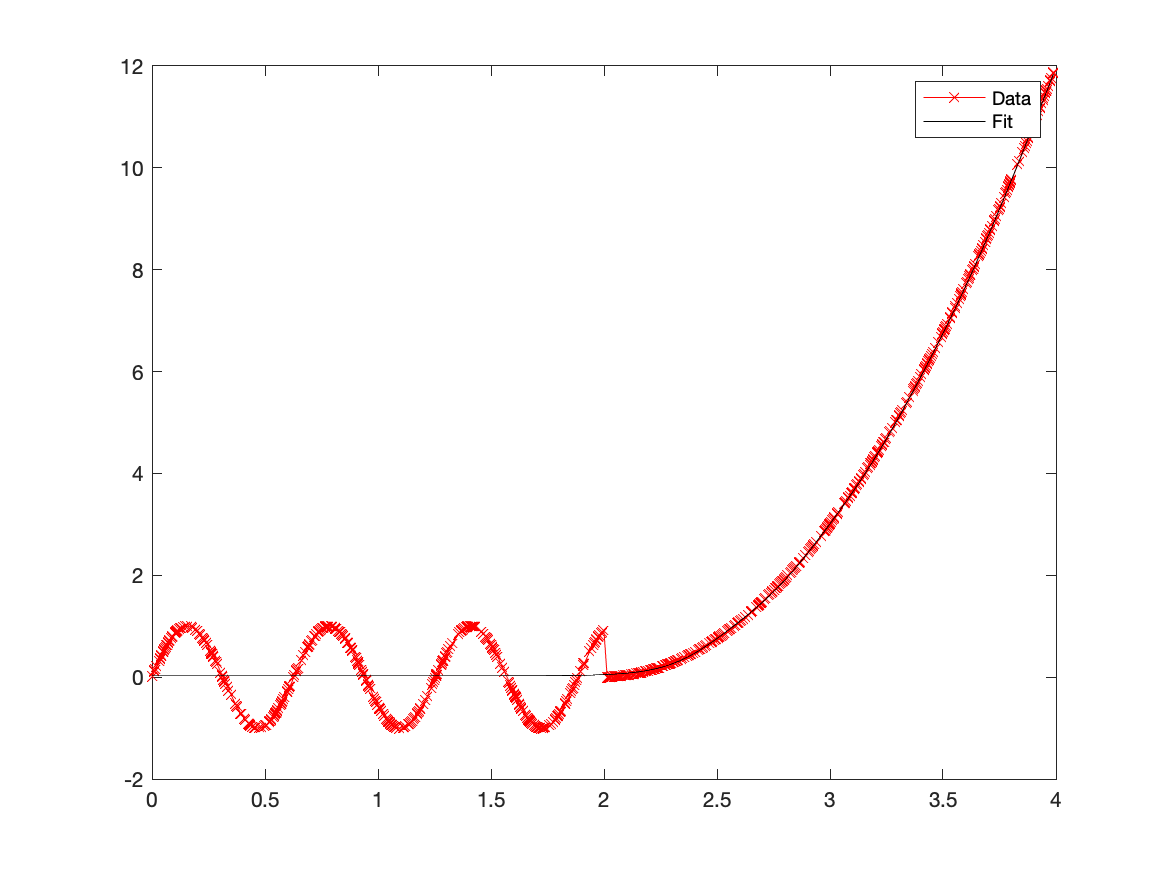
\includegraphics[scale=0.5]{NN_Example/Fig_Shallow_7.png}
\end{figure}
Got stuck at local minima!  (Bad!)
\end{frame}

\begin{frame}
\frametitle[alignment=center]{Neural Networks: 8 Logit+Linear Approx}
\begin{figure}
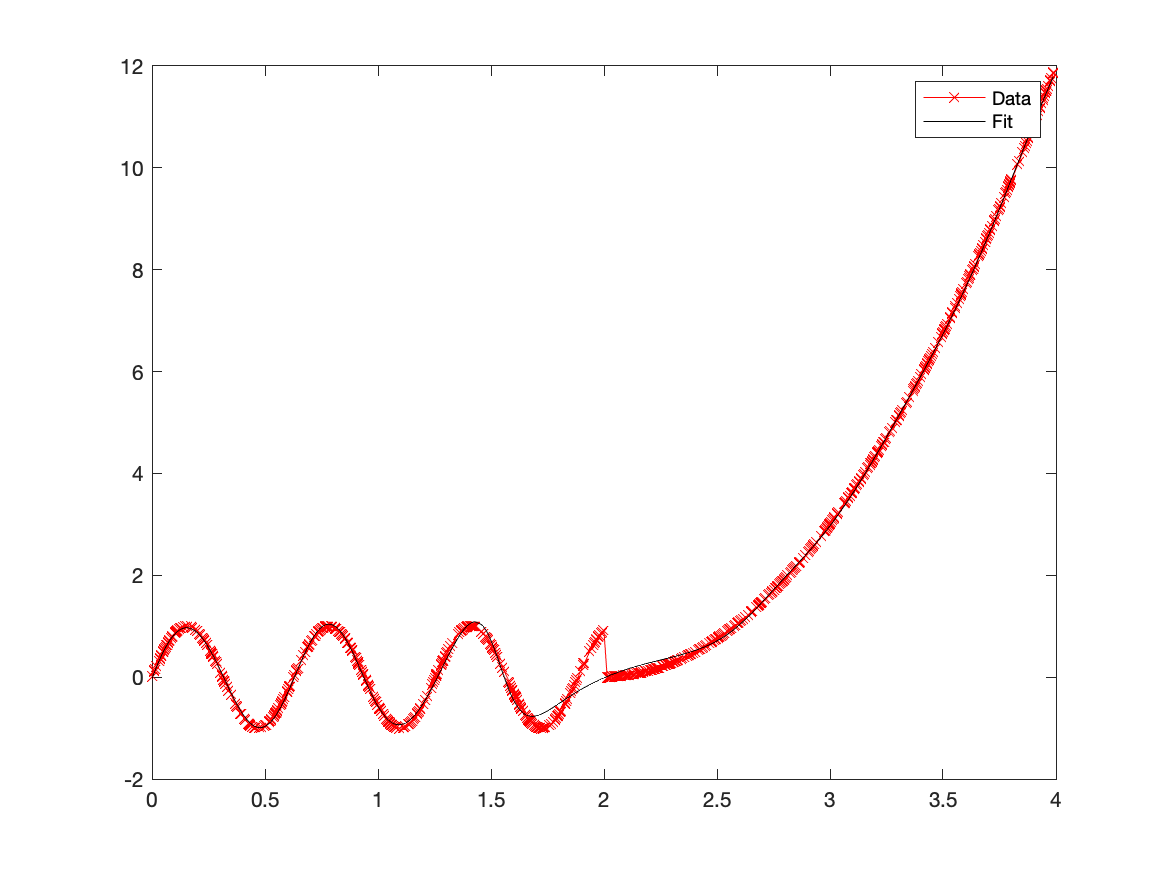
\includegraphics[scale=0.5]{NN_Example/Fig_Shallow_8.png}
\end{figure}
\end{frame}

\begin{frame}
\frametitle[alignment=center]{Neural Networks: 9 Logit+Linear Approx}
\begin{figure}
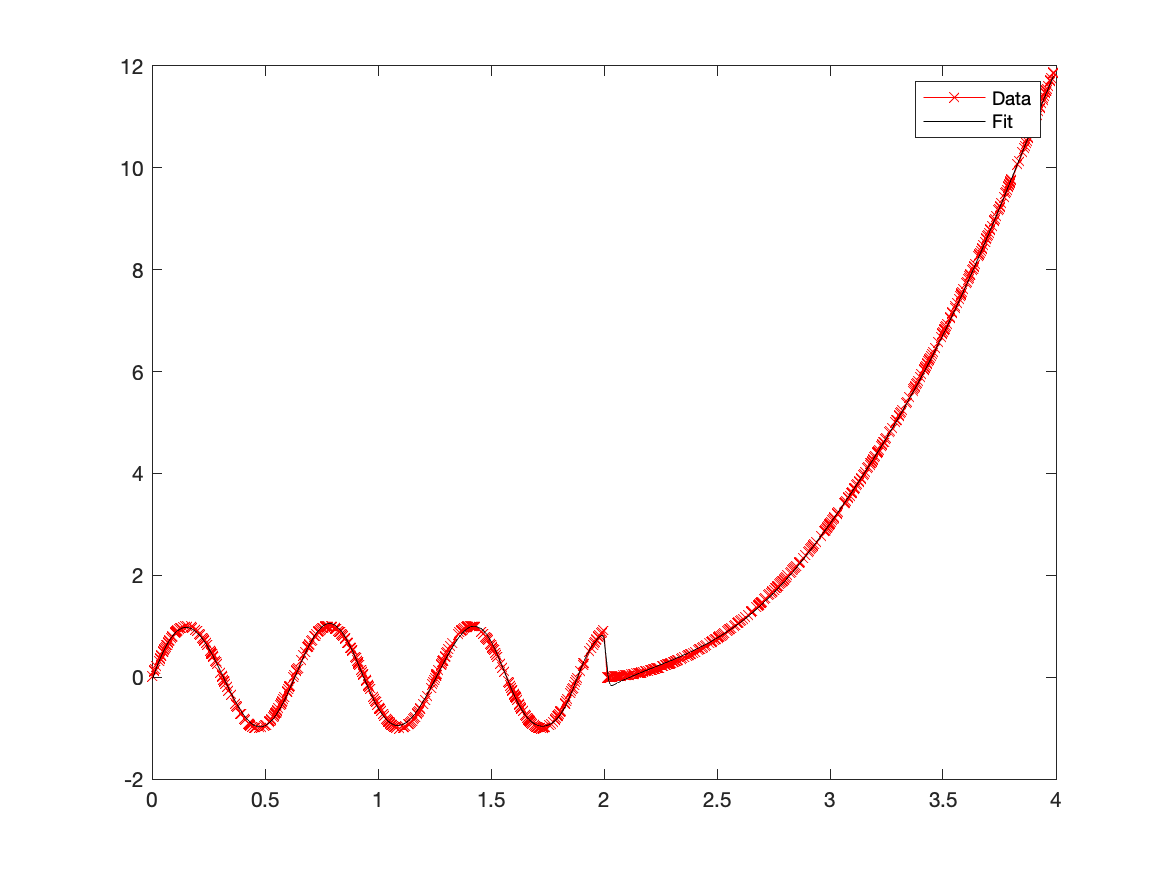
\includegraphics[scale=0.5]{NN_Example/Fig_Shallow_9.png}
\end{figure}
\end{frame}

\begin{frame}
\frametitle[alignment=center]{Neural Networks: 10 Logit+Linear Approx}
\begin{figure}
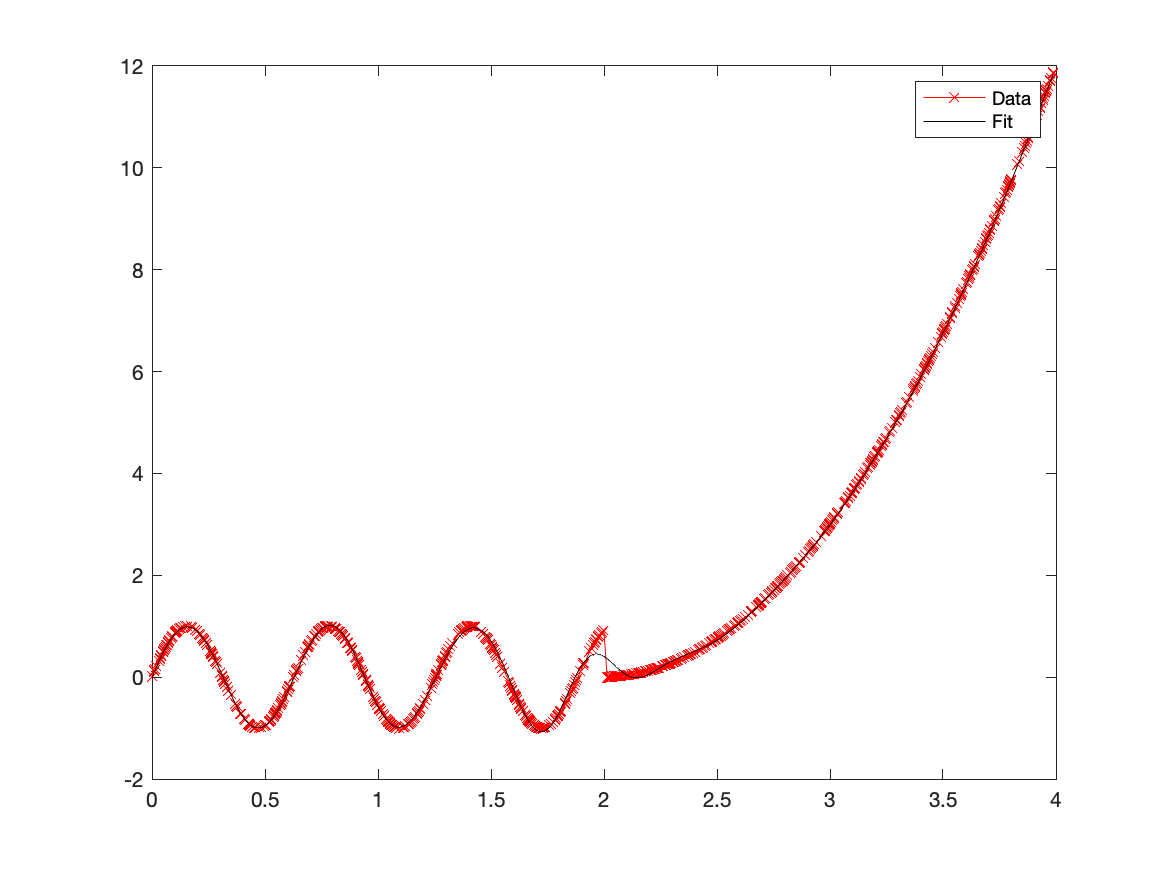
\includegraphics[scale=0.5]{NN_Example/Fig_Shallow_10.png}
\end{figure}
\end{frame}

\begin{frame}
\frametitle[alignment=center]{Neural Networks: 11 Logit+Linear Approx}
\begin{figure}
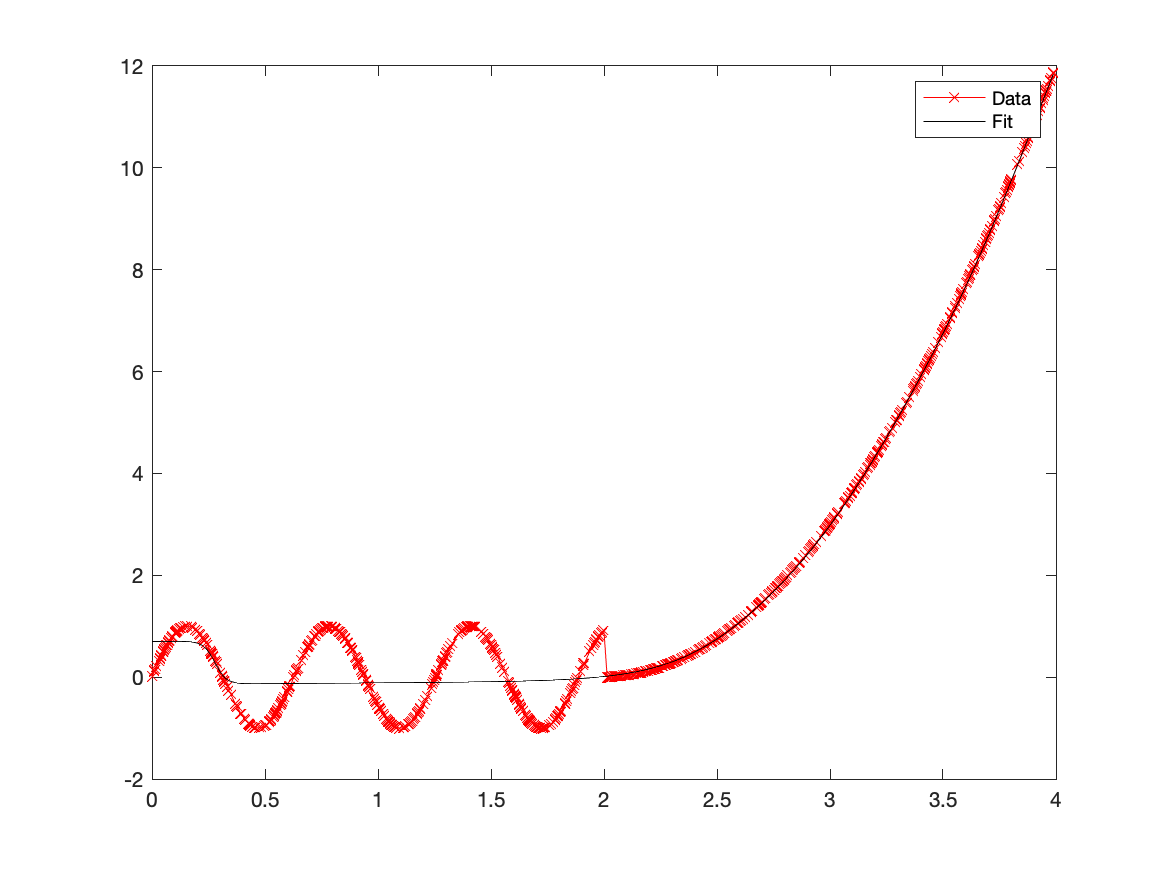
\includegraphics[scale=0.5]{NN_Example/Fig_Shallow_11.png}
\end{figure}
\end{frame}

\begin{frame}
\frametitle[alignment=center]{Neural Networks: 12 Logit+Linear Approx}
\begin{figure}
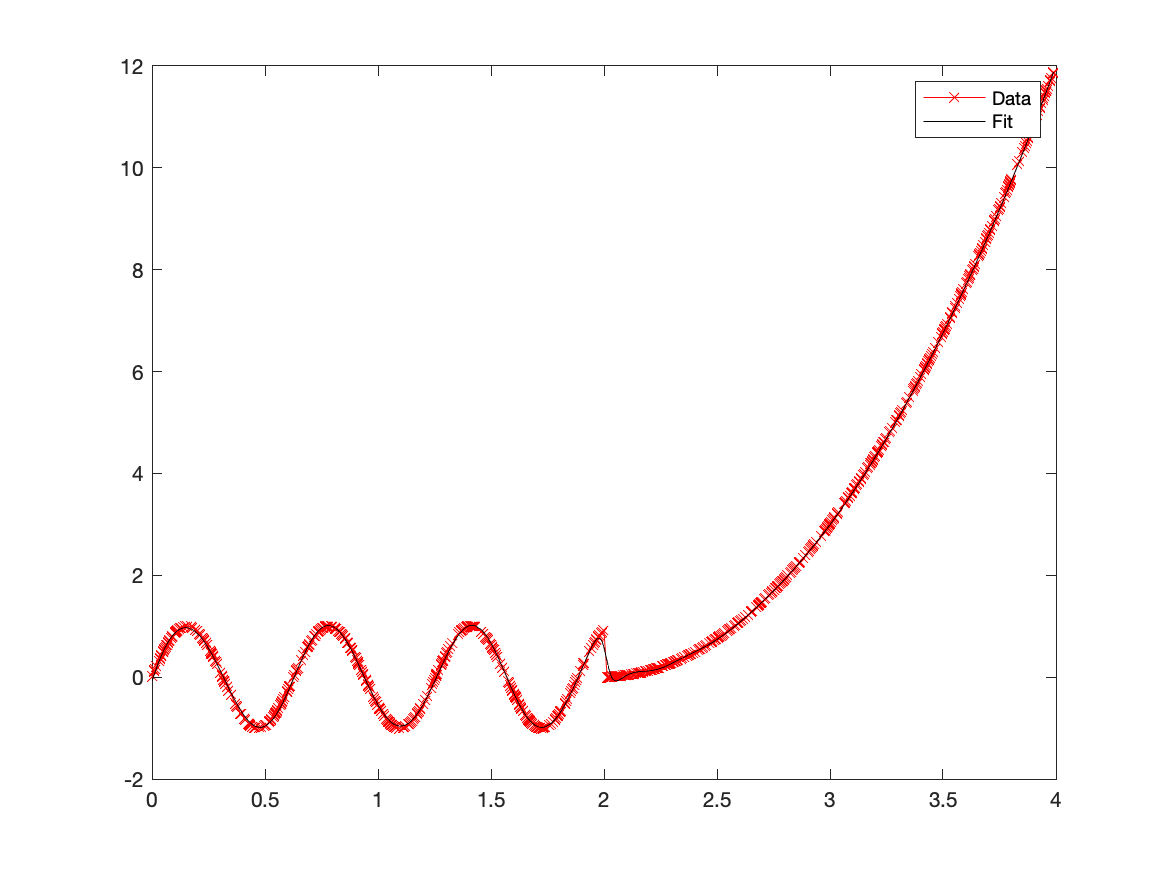
\includegraphics[scale=0.5]{NN_Example/Fig_Shallow_12.png}
\end{figure}
\end{frame}

\begin{frame}
\frametitle[alignment=center]{Neural Networks: 13 Logit+Linear Approx}
\begin{figure}
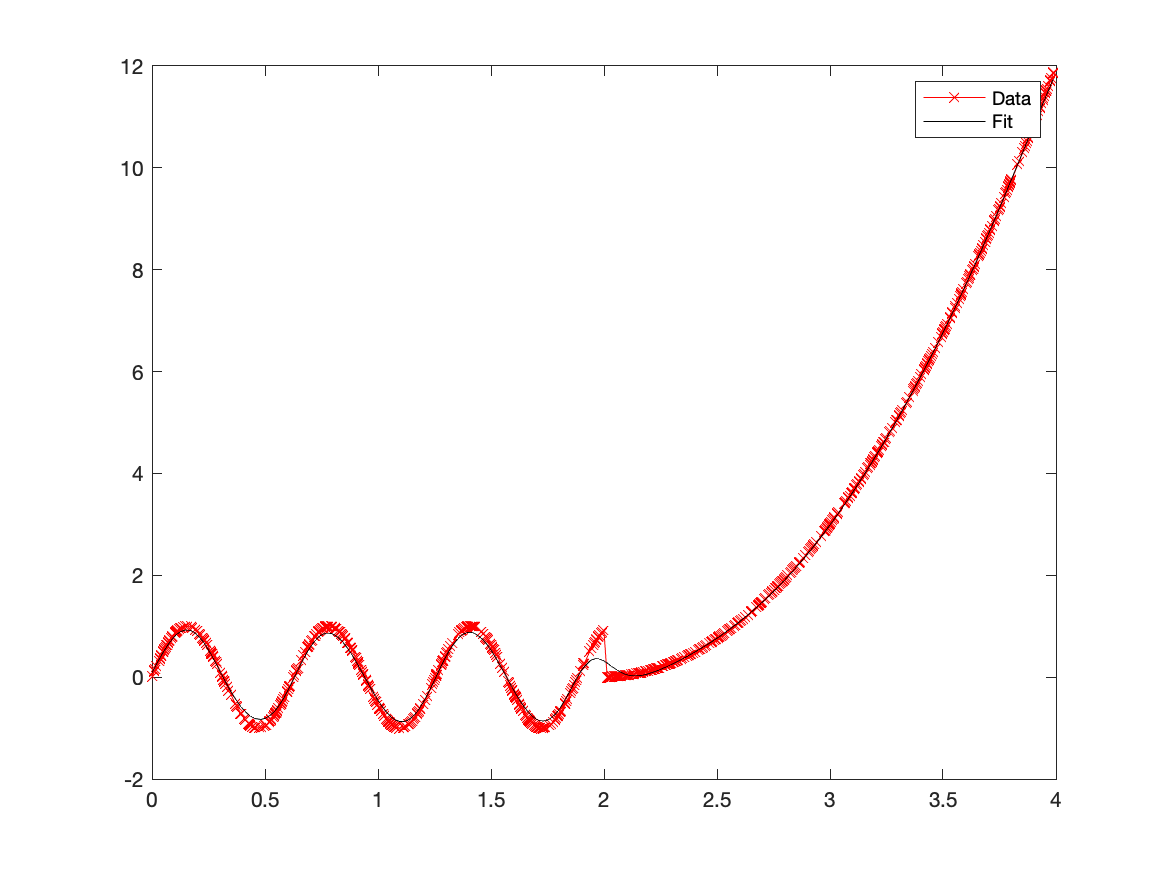
\includegraphics[scale=0.5]{NN_Example/Fig_Shallow_13.png}
\end{figure}
\end{frame}

\begin{frame}
\frametitle[alignment=center]{Neural Networks: 14  Logit+Linear Approx}
\begin{figure}
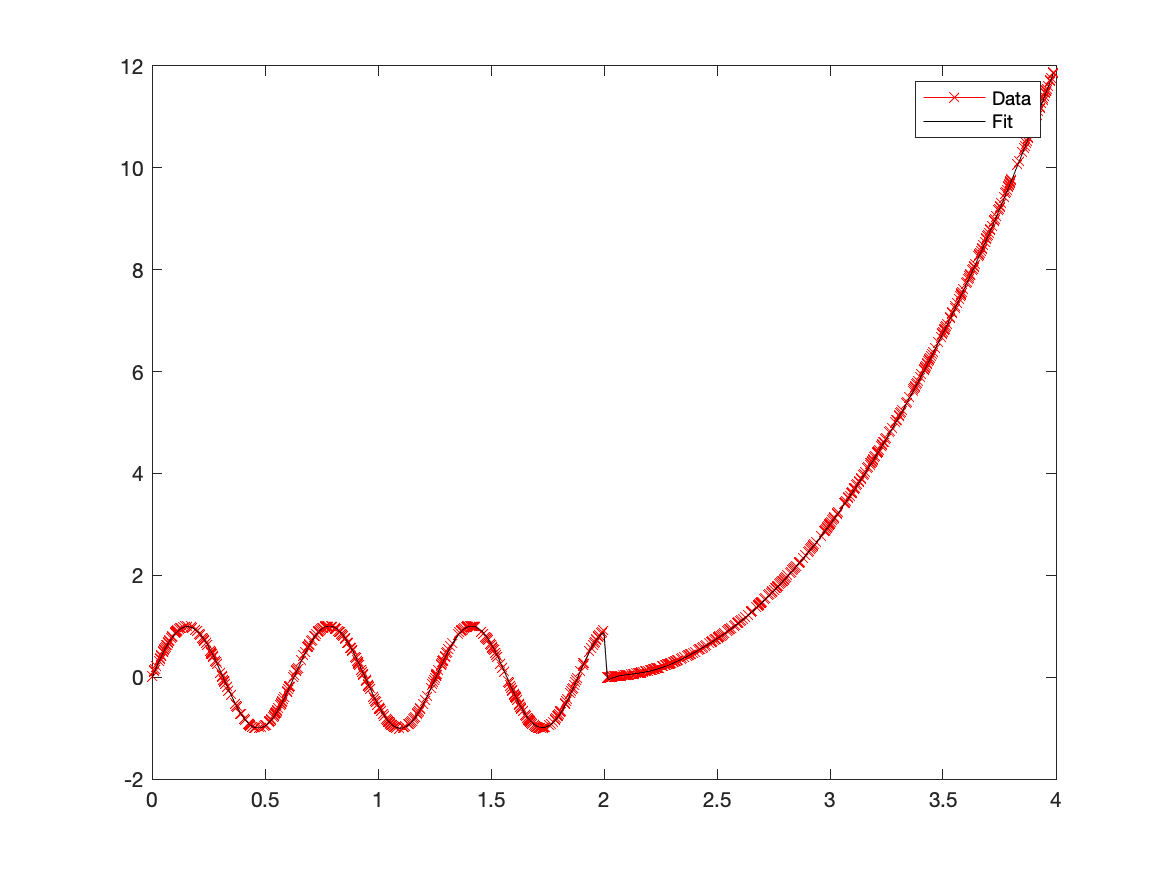
\includegraphics[scale=0.5]{NN_Example/Fig_Shallow_14.png}
\end{figure}
\end{frame}

\begin{frame}
\frametitle[alignment=center]{Neural Networks: 15 Logit+Linear Approx}
\begin{figure}
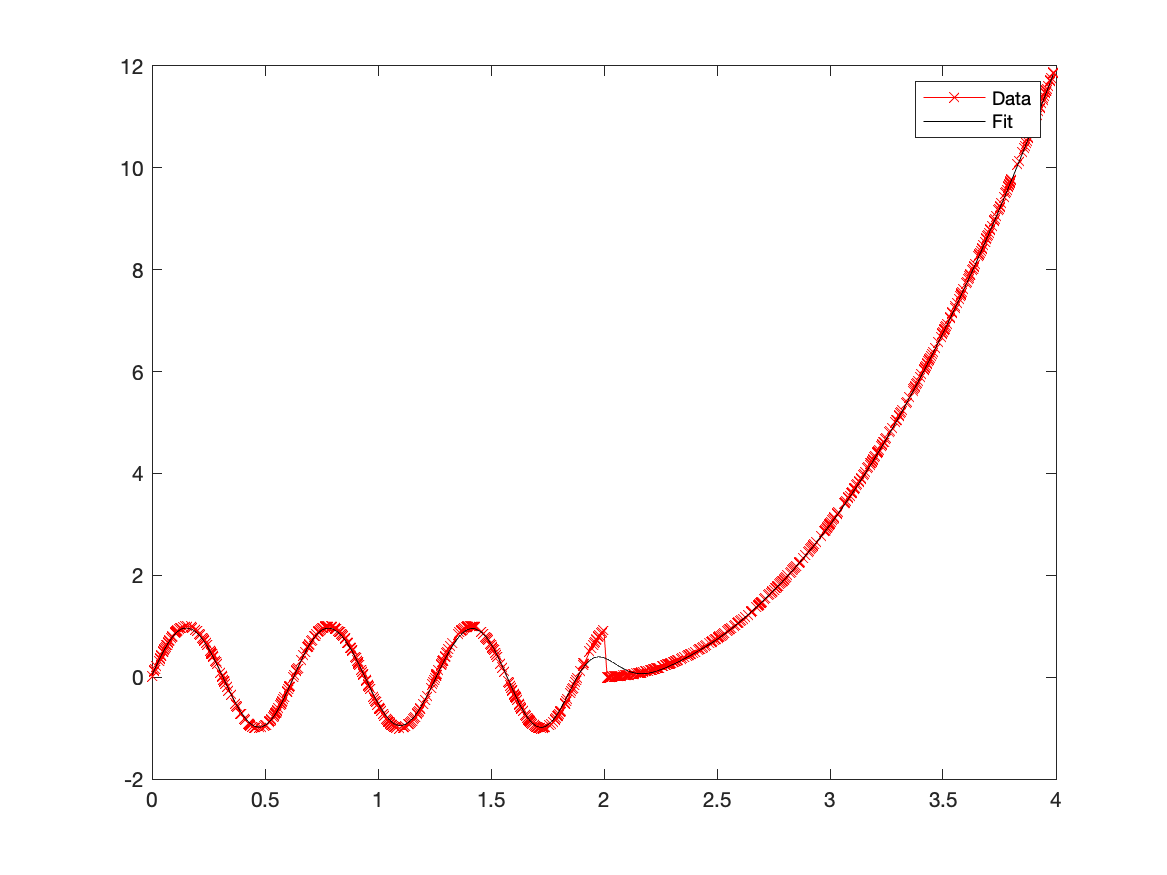
\includegraphics[scale=0.5]{NN_Example/Fig_Shallow_15.png}
\end{figure}
\end{frame}


\begin{frame}
\frametitle[alignment=center]{Deep Learning}
\begin{itemize}
\item I think of Neural Networks as really flexible sets of if statements combined with linear functions.
\bigskip
\item Logits act as "if's"
\bigskip
\item But could have a doubly-stacked if statement: 
\begin{itemize}
\item First layer: $$f_{a,1}(x_1,x_2)=1\iff x_1>3$$ $$f_{a,2}(x_1,x_2)=1\iff x_2<1$$
\item Second layer: $$f_b(f_{a,1},f_{a,2})=1\iff f_{a,1}==1\ \&\ f_{a,2}==1$$
\end{itemize}
\item Idea:  multiple layers give ability to encode complex ``if" statements ``easily"
\bigskip
\item Let's see my stacked version!  Deep\_N\_Main.m
\end{itemize}
\end{frame}

\begin{frame}
\frametitle[alignment=center]{Neural Networks: 5x5 Logit+Linear Approx}
\begin{figure}
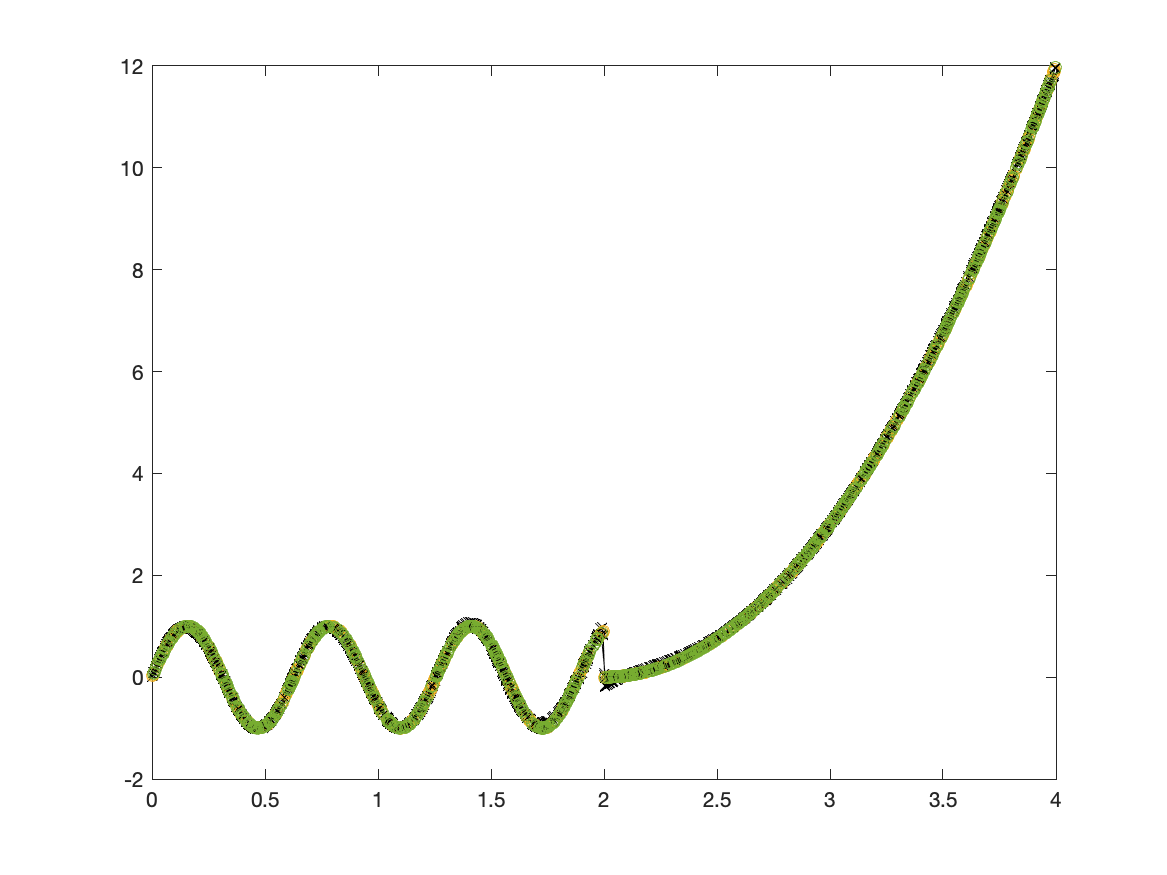
\includegraphics[scale=0.5]{NN_Example/Deep_7_7.png}
\end{figure}
\end{frame}


%\begin{frame}
%\frametitle[alignment=center]{Neural Networks: 20x10 Logit+Linear Approx}
%\begin{figure}
%\includegraphics[scale=0.5]{NN_Example/Deep_20_10.png}
%\end{figure}
%\end{frame}




\begin{frame}
\frametitle[alignment=center]{Neural Networks}
\begin{itemize}
\item Can generalize this, add more layers of logits or other functions
\item Because minimized with gradient descent, we want things that we can use chain rule on
\item Because multiple minima, want things that are bounded
\item Some common ones:
\begin{itemize}
\item ``Rectifier" $f(x)=max(0,x)$ (helps for piecewise)
\item Hyperbolic tangent $tanh(x)$ (similar to logit/``sigmoid", but -1 to 1)
\item Scaling layer: $\alpha+\beta X$
\item Softmax/``categorical distribution": vector output, takes vec $x$ and spits out $\frac{exp(x_i)}{\sum_j exp(x_j)}$
\item Less relevant in most econ: convolution, pool ``nearby" observations
\item LSTM: let value today affect fits for tomorrow (so $f(X_2)$ (X matrix at $t=2$) is a function of $X_2$ and $X_1$), all the way back
\item Dropout layer: randomly drop inputs (train drunk!)s
\end{itemize}
\end{itemize}
\end{frame}


\begin{frame}
\frametitle[alignment=center]{Matlab: build in shallow NN}
\begin{itemize}
\item Matlab has a lot of built-in neural network stuff
\bigskip
\item Unfortunately(?) this is an evolving field, and so commands are changing, becoming obsolete, etc.
\bigskip
\item Can be frustrating, but equivalent to Theano dying, Google transitioning from TensorFlow to JAX(?)
\bigskip
\item But can be as simple as:\\
\texttt{net = fitnet(netsize);}\\
\texttt{net = train(net,Xdata,Ydata,'UseParallel','yes');}\\
 \item Just like we write before, a bunch of logits that are netsize, give it X and Y data, minimizes.
 \bigskip
 \item Great for predicting, obviously \textbf{not solution for causality} (sorry micro ppl)
\end{itemize}
\end{frame}




\begin{frame}
\frametitle[alignment=center]{Example to fit:  $x.^2+y.^2-2sin(x.*y)$}
\begin{itemize}
\item See Fitnet Example/Main.m for details!
\end{itemize}
\end{frame}


\begin{frame}
\frametitle[alignment=center]{The Three Curses of Dimensionality}
\begin{itemize}
\item The three curses of dimensionality
\bigskip
\begin{enumerate}
\item As \textcolor{blue}{$n_{states}$} proliferates, \# problems to solve explodes for VFI
\smallskip
\item As \textcolor{red}{$n_{actions}$} proliferates, \# choices to compare explodes
\smallskip
\item As \textcolor{green}{$n_{outcomes}$} proliferates (particularly stochastic), space to integrate over explodes
\end{enumerate}
$$V(\textcolor{blue}{x})=\max_{\textcolor{red}{y\in\Gamma(X)}}\left\{F(x,y)+\beta \textcolor{green}{E(V(x'(y)))}\right\}$$
\item This is a problem if you're trying to model lifecycle behavior...age, permanent wage, transitory wage, marital status, age of kids, occupation, health, etc.
\bigskip
\item How can we solve?
\end{itemize}
\end{frame}


\begin{frame}
\frametitle[alignment=center]{One way to approximately solve the problem}
\begin{itemize}
\item There are many flavors of solution, but we'll focus on the ``Actor-Critic" method
\bigskip
\item Have two functions, parameterized by $\theta$ and $\phi$:
\begin{itemize}
\item Actor function $\overline{\pi}(y|x;\theta)$ takes in state and spits out an action (possibly probabilistically)
\bigskip
\item Critic function $\overline{Q}(x,y|\phi)$  takes in state and spits out value (Q-function, value function would be $\overline{V}(x|\phi)=\overline{Q}(x,\overline{\pi}(y|x;\theta)|\phi)$)
\end{itemize}
\bigskip
\item We can represent Actor \& Critic as flexible neural networks parameterized by $\theta$ and $\phi$ but how get values to fit?
\bigskip
\item Good actor function embeds both reward and stochastic future (actions and integral!)
\bigskip
\item \emph{Given} $\theta$ and $\phi$, can simulate an agent, get data to fit
\bigskip
\item Need to find $\theta$ and $\phi$
\end{itemize}
\end{frame}


\begin{frame}
\frametitle[alignment=center]{Actor-Critic Algorithm (\textbf{sketch(!)})}
\begin{itemize}
\footnotesize
\item Start with a guess for $\theta$ and $\phi$, and an initial state value
\item Simulate the system, get data
\item Now we have a bunch of paths for a given $\theta$ and $\phi$
\item Define ``disappointment" as difference between what we thought we would get and what we actually got, using our critic to fill in for the future:
$$D_t=reward_t+\overline{V}(x'|\phi)-\overline{Q}(x,y|\phi)$$
\item Update the critic to minimize the sum of squared errors between expectation and experience
$$d\phi=\sum_{t=1}^N\nabla_{\phi}(D_t(\phi))^2$$
\item Update the actor using the chain rule: $\theta$ affects $A$, $A$ affects $Q$.
$$d\theta=\sum_{i=1}^N\nabla_yQ(x,y;\phi)\nabla_\theta \overline{\pi}(y|x;\theta)  $$
\item Idea:  $d\theta$ pushes us in direction of better choices/happiness, $\nabla_{\phi}$ pushes us in direction of lower error in value function
\item Update the parameters of the functions:
$$\theta=\theta+\alpha d\theta$$
$$\phi=\phi+\beta d\phi$$
\item So we update the actor $\pi$ using critic $V$, and update $V$ using simulation
\end{itemize}
\end{frame}


\begin{frame}
\frametitle[alignment=center]{Detail on the Gradient}
\begin{itemize}
\item Let's say that $Q(x,y)=abs(y-x)$, and we know the true $Q$
\item So optimal action function is $y^*=x$ $\phi^{true}=\left[\begin{array}{c}0 \\ 1\end{array}\right]$
\item But we start with a bad action function: $y^*=0.5+2*x$.  $\phi=\left[\begin{array}{c}0.5 \\ 2\end{array}\right]$
\item We sample the point $x=1$, and choose $y=2.5$
\item Then $\nabla_yQ(x,y;\phi)=-1$, b/c linear penalty to missing target
\item And $\nabla_\theta=\left[\begin{array}{c}1 \\ 1\end{array}\right]$
\item Multiplying together, we get:
$$d\phi = \left[\begin{array}{c}-1 \\ -1\end{array}\right]$$
\item Then, if we put a weight of $0.01$ on the update we get:
$$\phi=0.99\left[\begin{array}{c}0.5 \\ 2\end{array}\right]+0.01\left[\begin{array}{c}-1 \\ -1\end{array}\right]=\left[\begin{array}{c}0.485 \\ 1.97\end{array}\right]$$
\item Closer to the truth!
\end{itemize}
\end{frame}



\begin{frame}
\frametitle[alignment=center]{Explaining to Mum-I}
\begin{itemize}
\item Start out with some surface that represents best action given state, and some surface that represents the value of being in that state
\bigskip
\item Simulate
\bigskip
\item Change value surface by comparing data with what you actually got (using initial surface for future, so change is slow), trying to match surface
\bigskip
\item Change action surface by trying to  increase received value vs value at best guess (small perturbations toward better actions)
\bigskip
\item Repeat in tiny steps
\end{itemize}
\end{frame}


\begin{frame}
\frametitle[alignment=center]{Idea}
\begin{itemize}
\item We try to toddle slowly to both how to evaluate our situation ($V$) and what to do ($\pi$)
\bigskip
\item We learn about value function by exploring the space
\bigskip
\item We learn about maximization (actor) by exploiting $V$ and our actual actions
\bigskip
\item We learn about expectation by simulation--enough simulations and we will explore the relevant space
\bigskip
\item Additional cool (but dangerous) aspect: we only explore relevant functions of state space
\bigskip
\item But how choose $V$ and $\pi$?
\end{itemize}
\end{frame}

\begin{frame}
\frametitle[alignment=center]{Choosing $V$ and $\pi$}
\begin{itemize}
\item $V$ and $\pi$ could be any functional form (e.g. linear $V=\alpha+\beta\sum_{j=1}^N\phi_jx_{j}$)
\bigskip
\item But we want an extremely functional flexible form
\bigskip
\item Neural networks are (typically) just simple stacked functions interacted with one another--think very flexilble functions, with many parameters
\bigskip
\item Advantage of NN-style flexibility is we can spend degrees of freedom in complicated areas and not in simple areas (as in sparse interpolation)
\bigskip
\item I'm giving this short shrift (sorry), but we'll put together a neural network for $V$ and $\pi$ in Matlab
\end{itemize}
\end{frame}

\begin{frame}
\frametitle[alignment=center]{Problem to Solve}
\begin{itemize}
\item We'll solve a simple finite-horizon NCG-style problem:
$$V(A,K,t)=\underset{\max}{K'}\left\{\log(A K^{\alpha}-K')+\beta E(V(A',K',t+1))\right\}$$
$$A'=(1-\rho)+\rho A+\epsilon,\ \ \ \epsilon\sim\mathcal{N}(0,0.05)$$
\item How will we set this up?
\bigskip
\item Define a set of functions that:
\bigskip
\begin{itemize}
\item A function that sets up actor and critic neural networks, defines observations, and trains (Main.m)
\bigskip
\item Initialize an agent (including random draws) (myResetFunction.m)
\bigskip
\item Step an agent forward in time, simulate draws (myStepFunction.m)
\end{itemize}
\end{itemize}
\end{frame}


\begin{frame}
\frametitle[alignment=center]{Reset Function}
\texttt{function [InitialObservation, LoggedSignal] = myResetFunction()}\\
\texttt{ \% Initial values}\\
\texttt{    S.K = 250+(rand(1,1)-0.5)*200;}\\
 \texttt{   S.A = 1+rand(1,1)*0.05;}\\
\texttt{    S.step = 1}   \\
 \texttt{  \% Return initial environment state variables as logged signals.}\\
\texttt{    LoggedSignal.State = [S.K;S.A;S.step];}\\
\texttt{    LoggedSignal.C=NaN;}\\
\texttt{    InitialObservation = LoggedSignal.State;}
\end{frame}

\begin{frame}
\frametitle[alignment=center]{Step Function}
\begin{itemize}
\item See myStepFunction.m
\bigskip
\item This is the simulator, it takes in signals and an action and simulates the environment, returns the observations, rewards, and whether or not it is done
\bigskip
\item Note:  logged signals are known to Matlab, but not agent.  Observations are known to agent.  In this simulation, they are the same thing.  (But could have had hidden state)
\end{itemize}
\end{frame}


\begin{frame}
\frametitle[alignment=center]{Main.m}
\begin{itemize}
\item See main.M
\bigskip
\item Idea:  set up a flexible function for the actor and critic, and then send to trainer
\end{itemize}
\end{frame}

\begin{frame}
\frametitle[alignment=center]{Comparing to Traditional VFI}
\begin{itemize}
\item There are many options to maximize, can take more time, etc.  but let's get a ballpark idea of how well this can do
\bigskip
\item Hard to see, so let's look at GraphDiff.m
\end{itemize}
\end{frame}

\begin{frame}
\frametitle[alignment=center]{Value Functions are Similar}
\begin{itemize}
\item There are many options to maximize, can take more time, etc.  but let's get a ballpark idea of how well this can do after five hours
\bigskip
\item Note: won't be perfect!  Feel free to run longer and/or with more parameters
\bigskip
\item Hard to see, so let's look at GraphDiff.m
\end{itemize}
\end{frame}

\begin{frame}
\frametitle[alignment=center]{Value Functions}
\begin{figure}
\centering
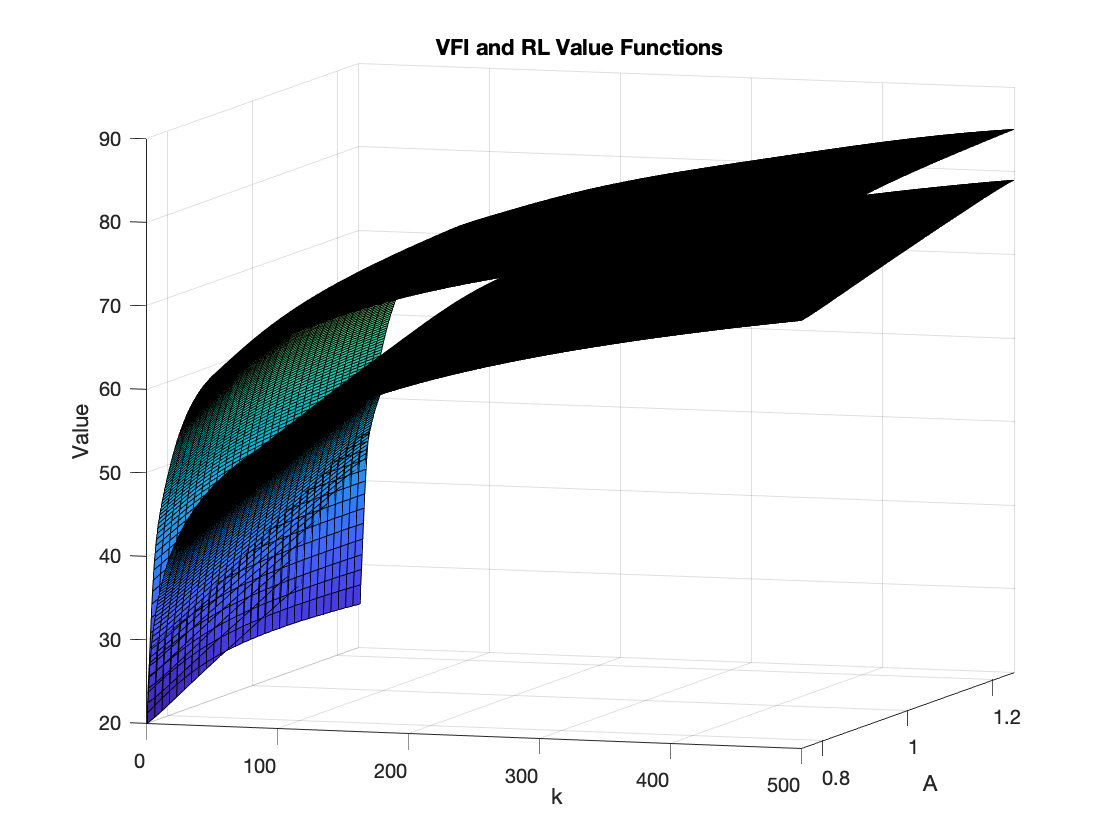
\includegraphics[scale=0.25]{Fig1.png}
\end{figure}
\end{frame}

\begin{frame}
\frametitle[alignment=center]{Policy Functions}
\begin{figure}
\centering
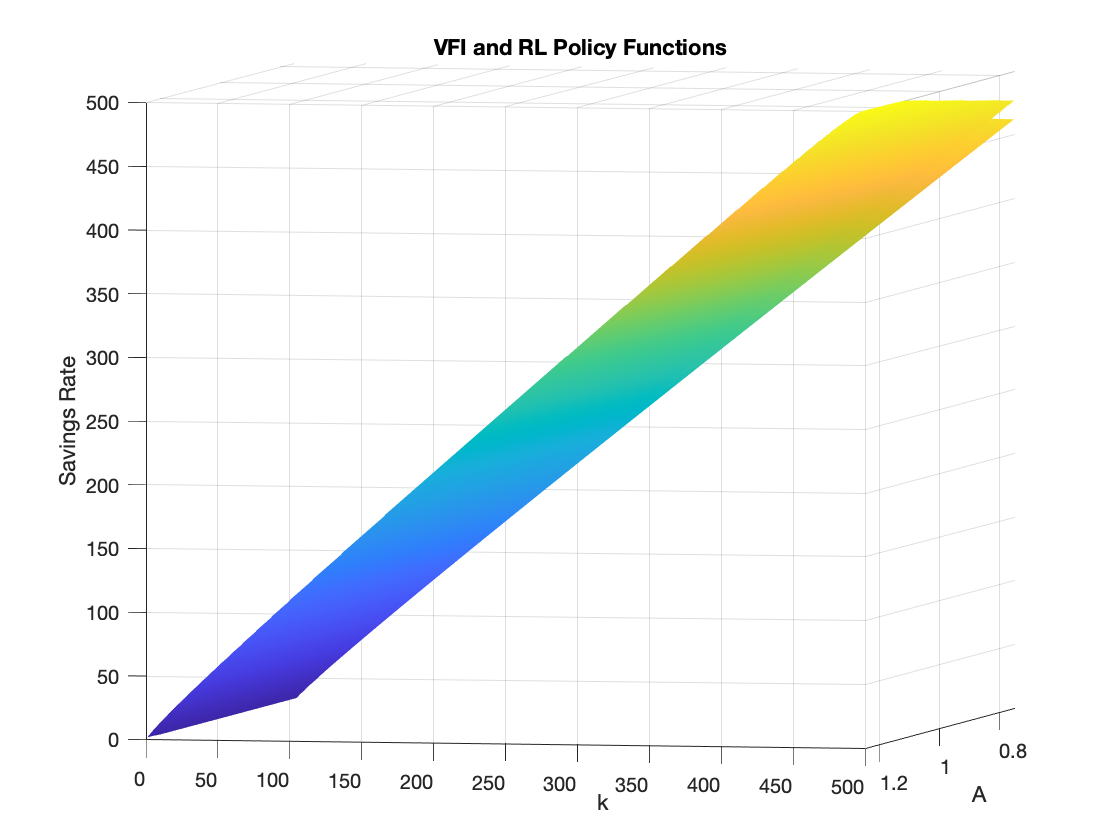
\includegraphics[scale=0.25]{Fig2.png}
\end{figure}
Hard to see, but right on top of one another
\end{frame}

\begin{frame}
\frametitle[alignment=center]{Policy Functions Difference}
\begin{figure}
\centering
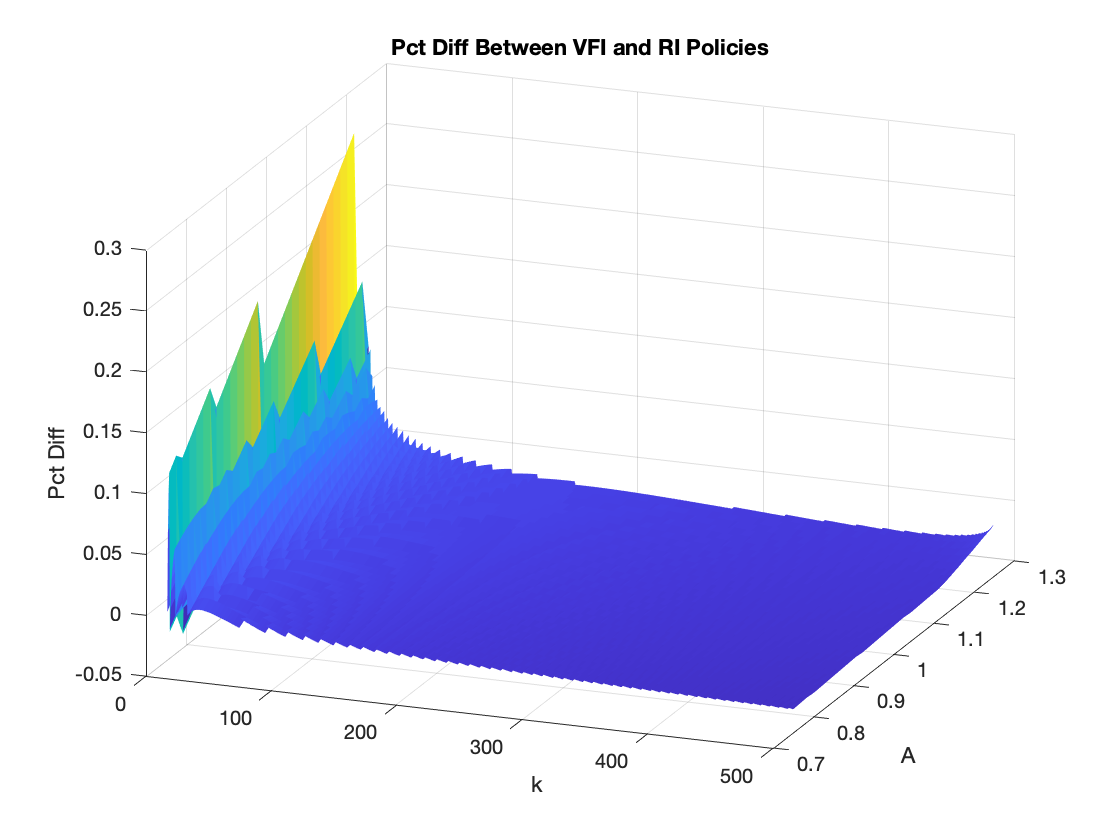
\includegraphics[scale=0.25]{Fig3.png}
\end{figure}
Mostly very small differences...except at k near zero (why?)
\end{frame}

\begin{frame}
\frametitle[alignment=center]{Simulation}
\begin{figure}
\centering
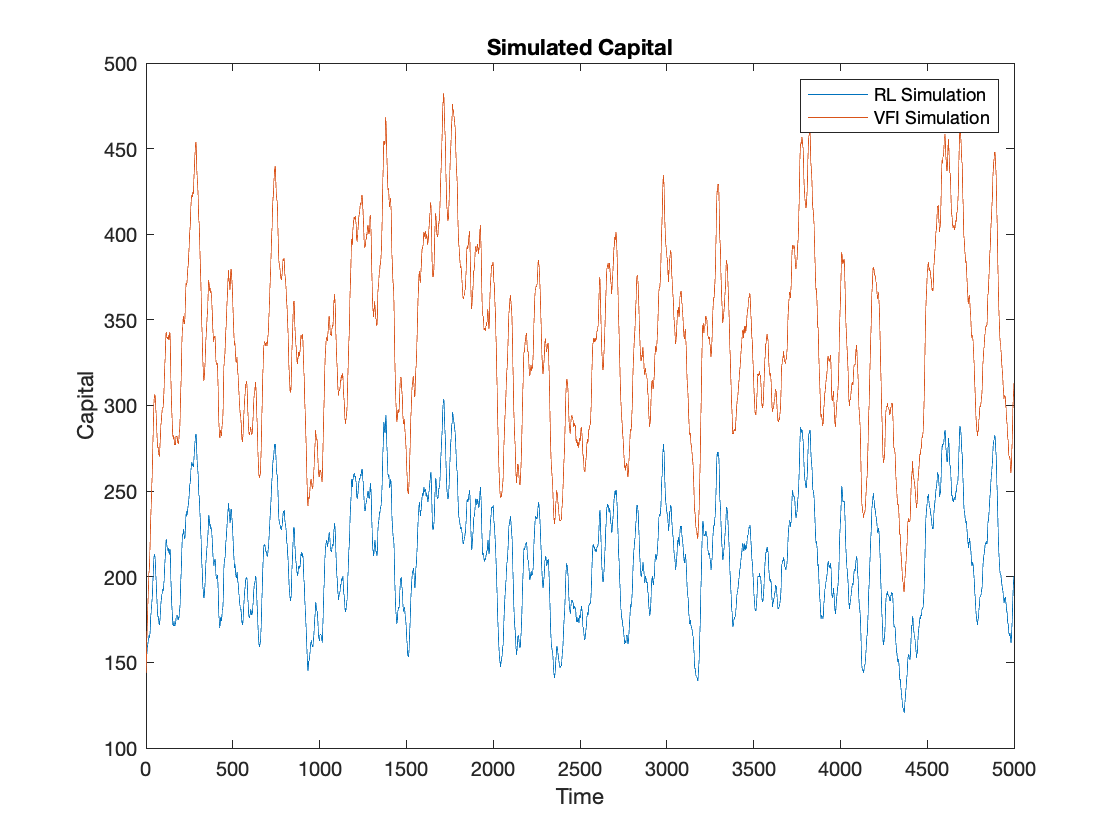
\includegraphics[scale=0.25]{Fig7.png}
\end{figure}
We get towards the right answer in percent deviations (let's check!)
\end{frame}


\begin{frame}
\frametitle[alignment=center]{Simulation}
\begin{figure}
\centering
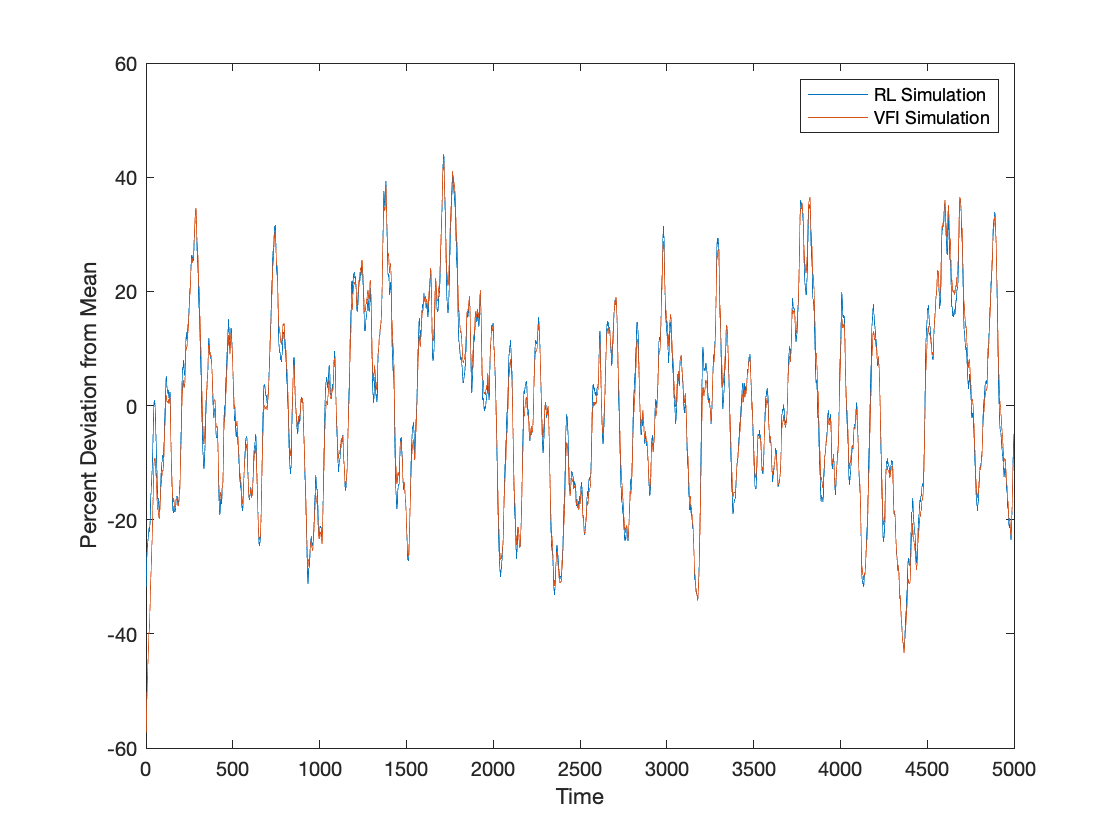
\includegraphics[scale=0.25]{Fig8.png}
\end{figure}
Mostly spot-on in differences
\end{frame}



\begin{frame}
\frametitle[alignment=center]{Simulation}
\begin{figure}
\centering
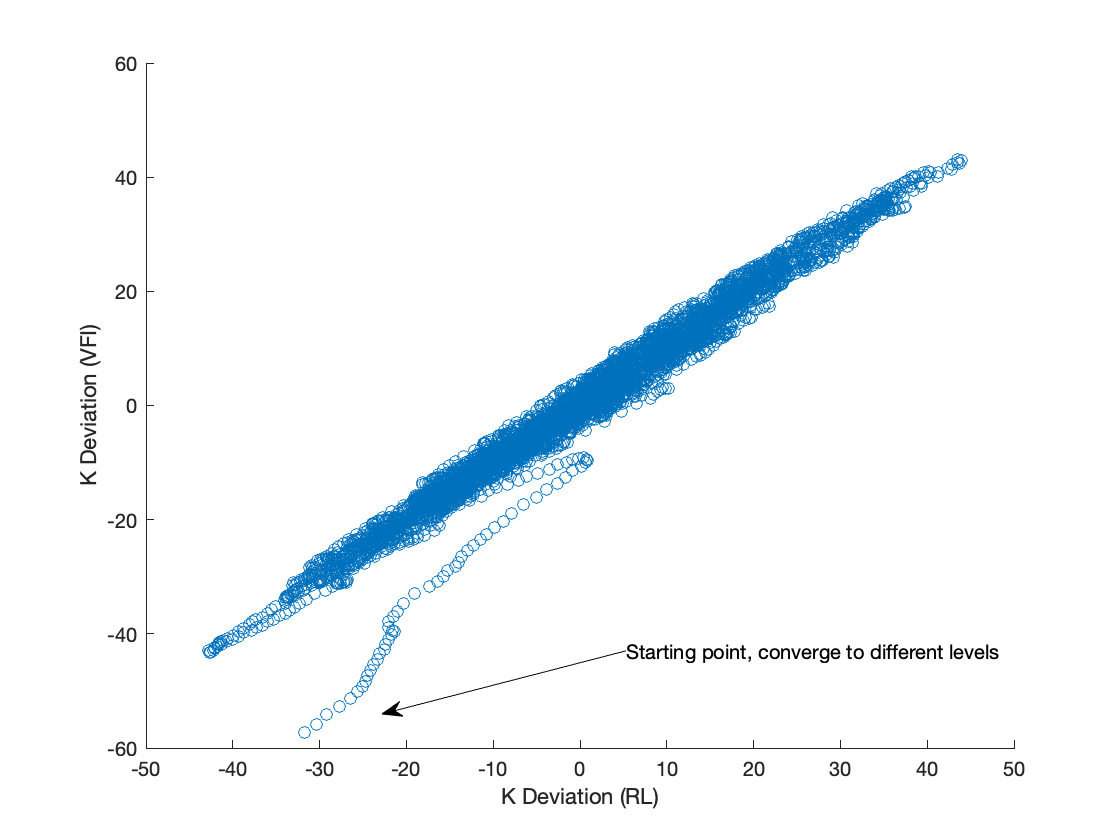
\includegraphics[scale=0.25]{Fig9.png}
\end{figure}
Not  terrible, but could use more running \& debugging to get level
\end{frame}




\begin{frame}
\frametitle[alignment=center]{We mostly sample points in the red area, so most accurate there}
\begin{figure}
\centering
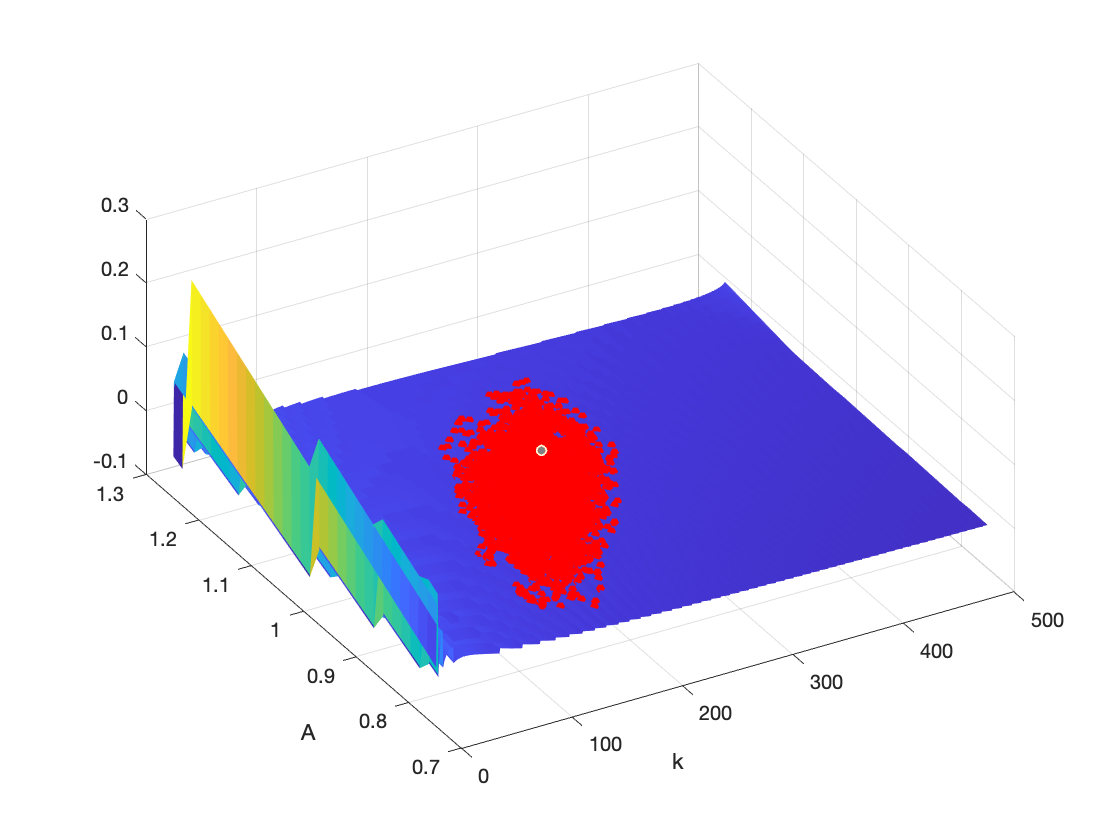
\includegraphics[scale=0.25]{Fig4.png}
\end{figure}
\end{frame}

\begin{frame}
\frametitle[alignment=center]{We mostly sample points in the red area, so most accurate there}
\begin{figure}
\centering
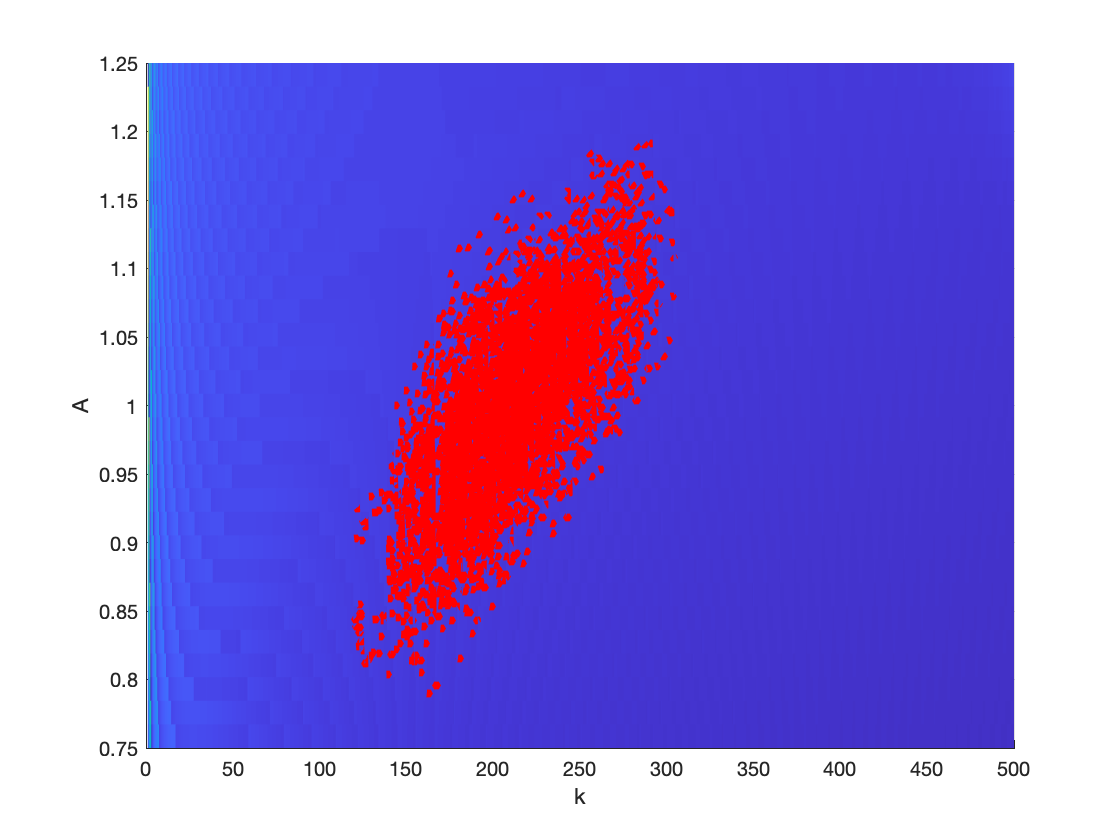
\includegraphics[scale=0.25]{Fig5.png}
\end{figure}
\end{frame}

\begin{frame}
\frametitle[alignment=center]{Some useful bounds}
\begin{figure}
\centering
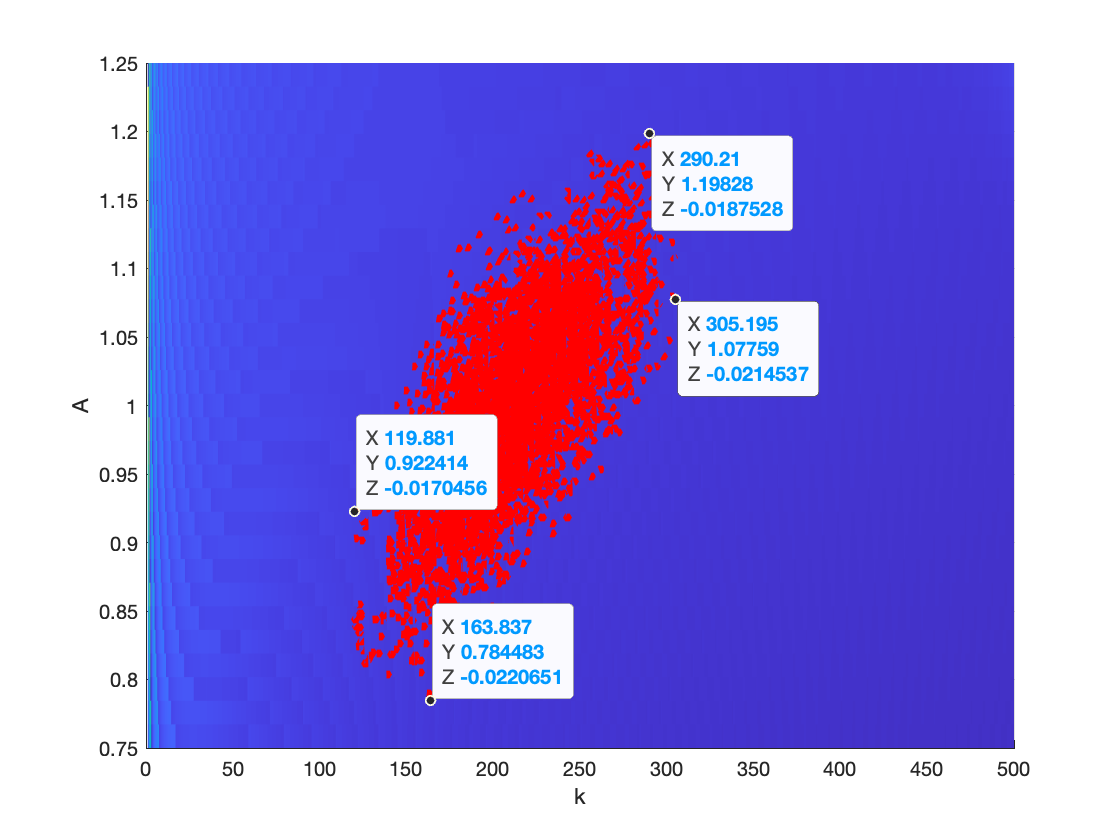
\includegraphics[scale=0.25]{Fig6.png}
\end{figure}
\end{frame}


\begin{frame}
\frametitle[alignment=center]{Summing Up}
\begin{itemize}
\item Reinforcement learning incredibly useful
\bigskip
\item Nothing spectacularly clever, just a combination of:
\begin{itemize}
\item Flexible functional forms (so many state variables can be accomodated efficiently)
\item \emph{Forward}-looking (average over many simulations is estimation)
\item Simple maximization (use gradient and flexible function, so don't have to solve perfectly and solutions potentially informative across state space)
\end{itemize}
\item Could have gone much farther.  Could have had parameters $\alpha$, $\rho$, etc. be draws too (solve not only over $k$ and $A$ but over parameterization, so can solve for heterogeneous agents or estimate parameters easily! (VFI would require solving for each parameter set).  
\bigskip
\item In practical terms, you just have a setup function, and then a function that steps through time (simulates) and pass it off to solver
\end{itemize}
\end{frame}


\begin{frame}
\frametitle[alignment=center]{Last warning}
\begin{itemize}
\item There's a lifetime of details in terms of efficiency, problem setup, solvers, etc., and the devil is in the details
\begin{itemize}
\item Discrete, continuous
\item Shallow RL, deep RL (how setup?)
\item On/off policy
\item Delayed learning
\end{itemize}
\bigskip
\item We went through one algorithm (actor-critic) and one example (continuous state \& action space).  
\bigskip
\item There are a cornucopia of flavors \& algorithms--I haven't yet found one that isn't intuitive \& obvious in retrospect (once you grok the core idea behind approximate dynamic programming idea)
\bigskip
\item However, economist notation and ML notation diverge a bit, so there's an investment in learning
\end{itemize}
\end{frame}

\begin{frame}
\frametitle[alignment=center]{Other ML Topics}
\begin{itemize}
\item We talked about reinforcement learning: have a problem, throw it at computer over and over, have computer solve it
\bigskip
\item There are other things you might care about:  highly nonlinear functions more generally (Kriging/gaussian process regression ``fitrgp")
\bigskip
\item Classification learning (such as support vector machines ``fitcsvm")
\bigskip
\item Regression learner
\bigskip
\item We won't talk about these, instead we'll start applying!
\end{itemize}
\end{frame}



\end{document}